\documentclass[11pt]{article}

\usepackage{sectsty}

% Margins
\topmargin=-0.45in
\evensidemargin=0in
\oddsidemargin=0in
\textwidth=6.5in
\textheight=9.0in
\headsep=0.25in

\title{Interactive Visualization}
\author{Joseph Weibel}
\date{\today}

\setcounter{secnumdepth}{-\maxdimen} % remove section numbering

\usepackage{url}
\usepackage[style=apa,backend=biber]{biblatex}
\addbibresource{bibliography.bib}
\setcounter{biburllcpenalty}{7000}
\setcounter{biburlucpenalty}{8000}

\usepackage{caption}
\captionsetup[figure]{font=tiny}

\usepackage{multicol}

\usepackage{wrapfig}
\usepackage{graphicx}
\makeatletter
\def\maxwidth{\ifdim\Gin@nat@width>\linewidth\linewidth\else\Gin@nat@width\fi}
\def\maxheight{\ifdim\Gin@nat@height>\textheight\textheight\else\Gin@nat@height\fi}
\makeatother
% Scale images if necessary, so that they will not overflow the page
% margins by default, and it is still possible to overwrite the defaults
% using explicit options in \includegraphics[width, height, ...]{}
\setkeys{Gin}{width=\maxwidth,height=\maxheight,keepaspectratio}
% Set default figure placement to htbp
\makeatletter
\def\fps@figure{htbp}
\makeatother

\usepackage{fancyhdr}
\pagestyle{fancy}
\fancyfoot[L]{Joseph Weibel}
\fancyfoot[R]{Interactive Visualization}

\begin{document}
\begin{titlepage}
    \begin{center}
        \vspace*{0.4cm}

        \Huge
        \textbf{Interactive Visualization}

        \vspace{0.3cm}
        \LARGE
        Report

        \vspace{0.8cm}

        \textbf{Joseph Weibel}

        \vfill

        % TODO image

        \vfill

        \vspace{0.3cm}

        \Large
        FHNW\\
        Data Science\\
        June 2022

        \vspace{1.0cm}

        \normalsize
        Github Repository: https://github.com/josefweibel/ds-ivi-report

        \vspace{0.8cm}

    \end{center}
\end{titlepage}
\pagebreak

\tableofcontents
\pagebreak

Visualisations are a great way to explore data and underpin statements with facts. While static ones are suitable for most cases, interactive plots allow showing more information in the space and allow the viewer to explore the data on their own. These plots can show additional information when the user moves their cursor over one of the data points, or they allow the users to compile their graphics as they like. However, creating such interactive visualisations requires detailed understanding to achieve good usability and avoid confusing the viewers. The following pages will outline theoretical aspects along with practical experience gathered while creating two dashboards created for project works in my studies. One visualises different measurements of a solar energy plant to inspect and compare these. While this is rather technical, the other one shows insights after exploring and comparing data of dementia patients with non-dementia people ~\parencite{alzheimers_disease_neuroimaging_initiative_adni_2022}.

\section{Performance}

Interactive visualisations tend to show more attributes and observations than static ones, which increases the risk of performance issues. Moreover, since users can influence its rendering, they need to be rerendered mostly after each interaction. On the other hand, static plots will be rendered once only when they are created. Then, when users want to see them, only a stored file must be shown to them, which computers nowadays can do in a few milliseconds.

The more data to show, the more likely it is that the visualisation suffers under long waiting times and thus the chance that viewers lose interest in the graphic. Especially if viewers need to wait after every interaction, the visualisation can be described as unusable. However, the actual latency is very likely to vary from computer to computer since it depends on the computing power and thus on the computer's hardware. Therefore it is difficult to say from how many data points and features performance issues may arise. Furthermore, performance issues may arise in different parts of creating a plot.

\begin{figure}
    \centering
    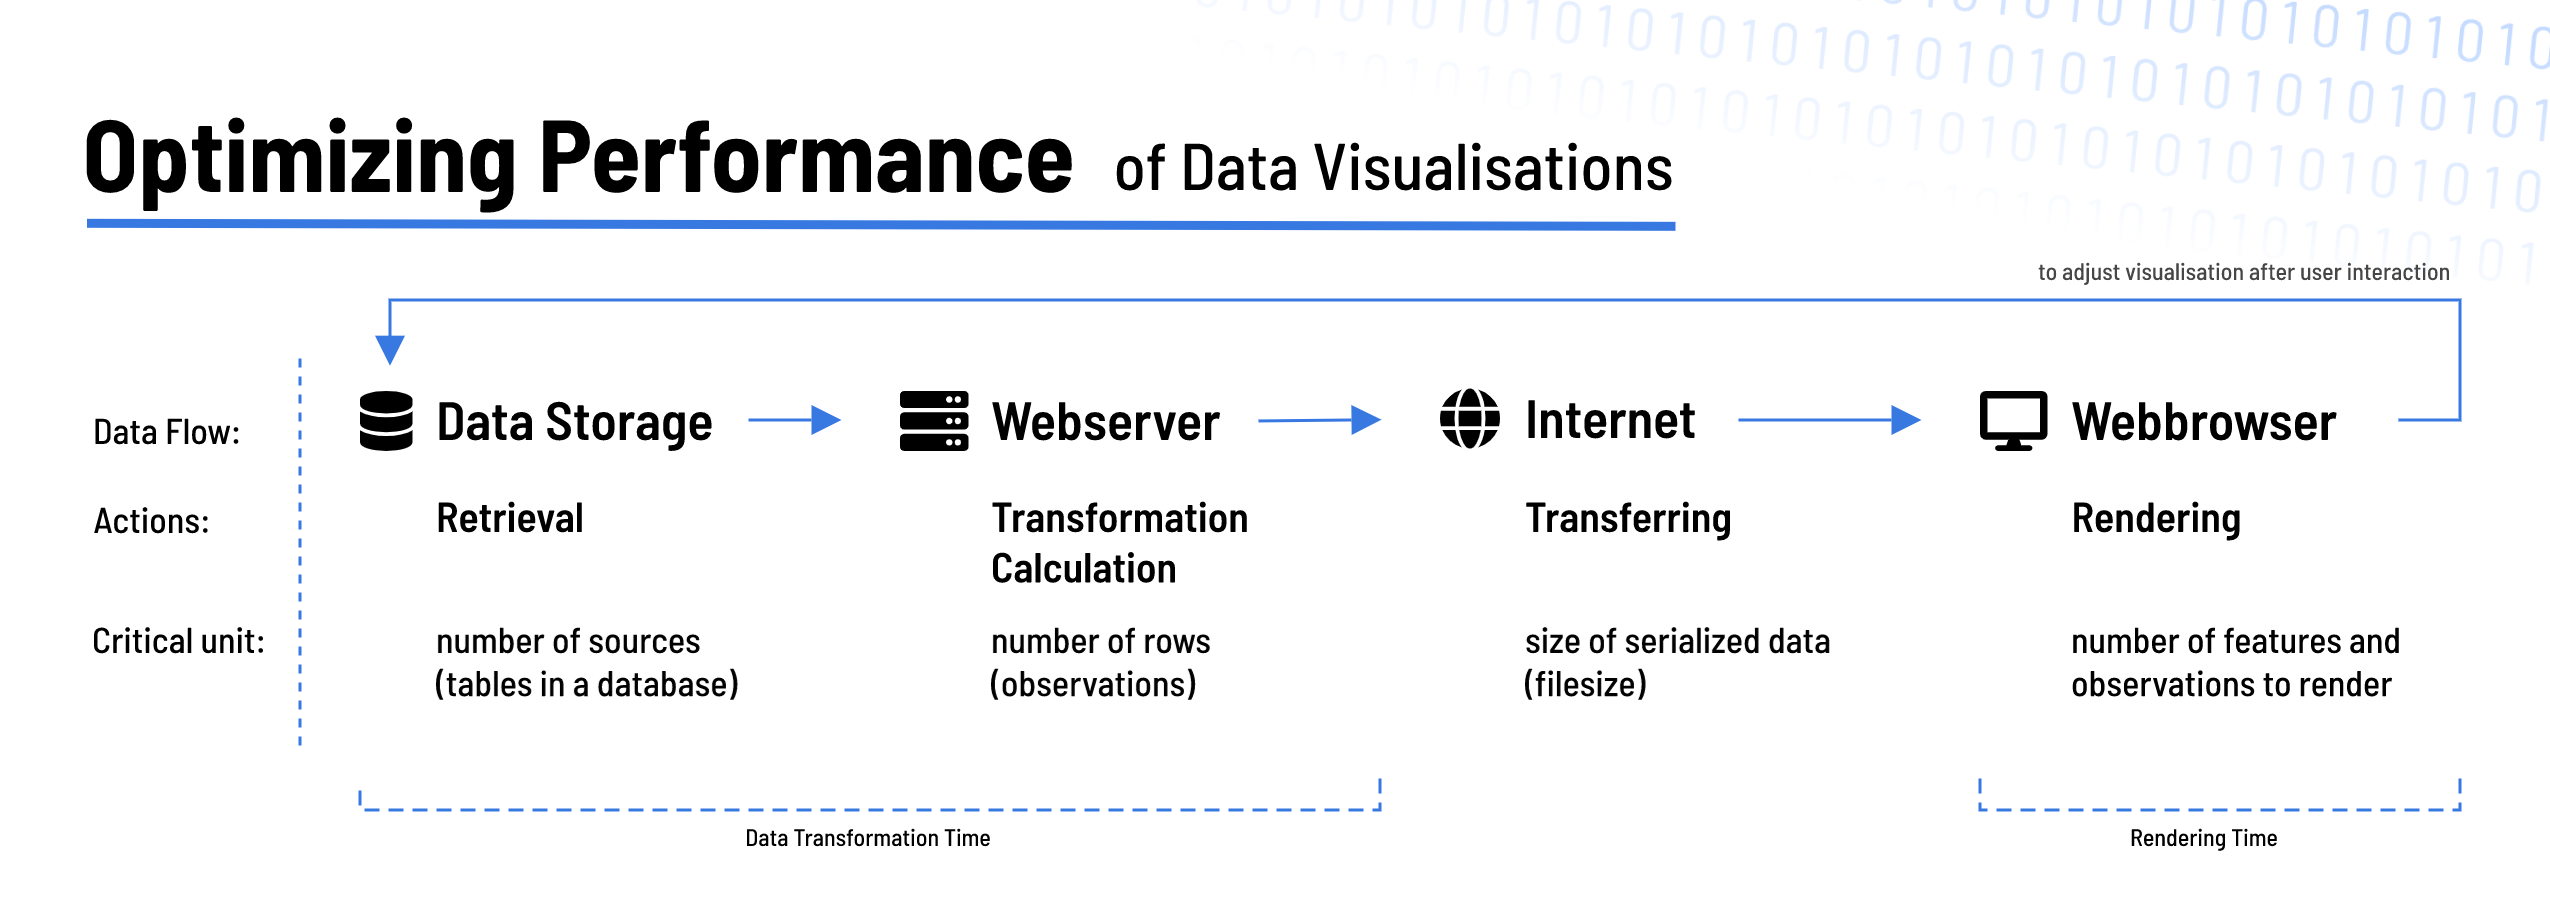
\includegraphics[width=0.7\textwidth]{./performance.png}
    \caption{Infographic showing process to build an interactive visualisation using web technologies. (own graphic)}
\end{figure}

\textit{Figure 1} visualises the four rough parts involved in interactive visualisations built with web technologies. In general, the more data, the more problematic, but the number of sources has a higher impact on data storage systems like databases than the number of features and rows. For example, to transfer data from the webserver to the web browser, only the filesize and the number of requests sent to the server matter. So it is irrelevant if the data consists of a vast amount of rows or attributes. More features affect the web browser's speed slightly more than the webserver since the browser has to add a separate component to the visualisation for every additional feature. Important to know that many web visualisation tools trigger the whole process after most human interactions with the plots.

\subsection{Measurements}

The performance of a visualisation can be quantified by using one of many possible metrics. It is either possible to measure specific overall timeframes or go a step further and use instrumentation to measure individual code blocks \parencite{isaacs_state_2014}. In web development, a tool called \textit{Lighthouse} \parencite{google_lighthouse_2021} has become the way to measure the performance of websites. It can also be applied to pages containing interactive visualisations and measures specific times like the number of seconds until the user can interact with the site (\textit{Time to Interactive}) or to the point when the first pixel is drawn on it (\textit{First Contentful Paint}).

\begin{wrapfigure}{R}{0.3\textwidth}
    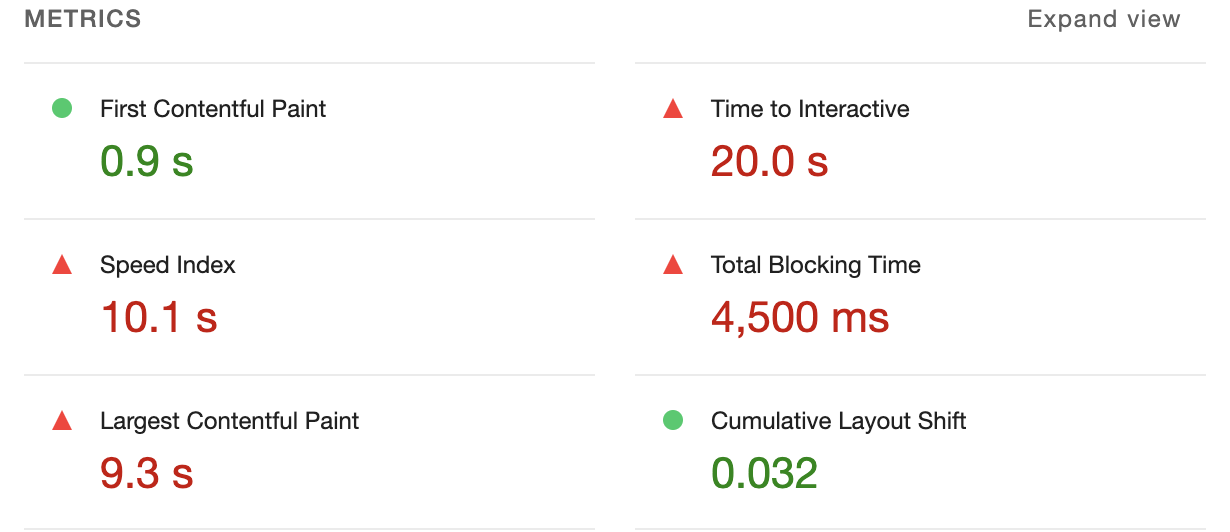
\includegraphics[width=0.3\textwidth]{./lighthouse-1.png}
    \caption{Lighthouse report for dashboard with all observations visible.}
\end{wrapfigure}

The dashboard for the solar energy plant's data suffered severe performance issues. It took quite some time until it got loaded and usable, but each time users changed one of the filters, they had to wait several seconds again for the updated plot. The Lighthouse report (see \textit{Figure 2}) confirms this impression. The total blocking time indicating the cumulated time the user had to wait until the page has been rendered completely is at 4.5 seconds, and the plots have been ready only after 20 seconds. This is too long for a tool to quickly get insights into the data.

\subsection{Solutions}

The possible solutions for slow visualisations are diverse and depend heavily on the problem. If the creation of a plot is deferred because of heavy computations or complex rendering, then outsourcing these tasks to the \textbf{Graphics Processing Unit (GPU)} can speed them up significantly. However, these improvements depend heavily on the available hardware, which is predominantly out of control for data scientists regarding the viewers' machines. For complex visualisations on websites, technologies like \textit{WebGL} should be used, which makes use of the GPU \parencite{mozilla_webgl_2022}.

When showing interactive maps, a technique called \textbf{Tiling} is often used to divide the enormous map into small images to be able to load only the images which are currently in the viewport and required for the current zoom level. This strategy can also be used for other visualisations. For the ones on websites, a library called \textit{Leaflet} is available \parencite{noauthor_leaflet_2022}.

When calculations after user interactions are not too complex, another improvement is avoiding server roundtrips and recalculating directly in the web browser. However, this is not always possible, primarily when a high-level framework like \textit{Dash} is used. If these can not be bypassed, it is advisable to check for data that can be \textbf{cached}. For example, the ADNI dashboard reloaded the source data on every filter change, which delayed the response by some seconds. However, since the data does not change, it could only be loaded once, and the delay could be removed.

\begin{wrapfigure}{R}{0.3\textwidth}
    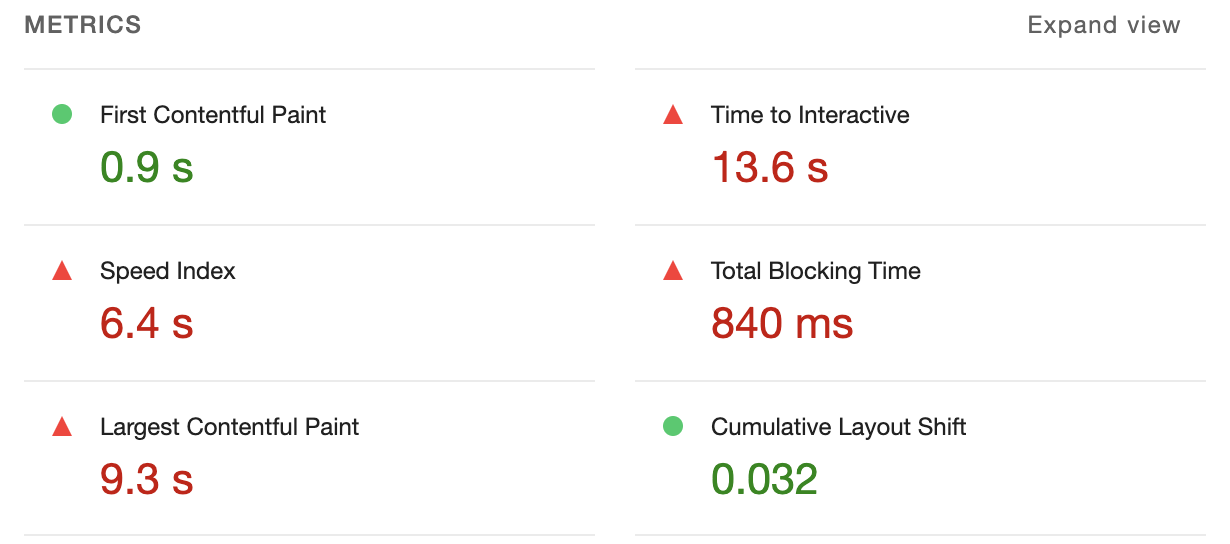
\includegraphics[width=0.3\textwidth]{./lighthouse-2.png}
    \caption{Lighthouse report for dashboard with only observations of one month visible.}
\end{wrapfigure}

Loading data only for one month instead of the complete dataset, which consists of 84'212 observations and 274 attributes, could improve the speed of the energy dashboard. This seemed like a good solution since that much data is overwhelming for the user anyway. Viewers can now switch between months using a filter. Such \textbf{filters} and reducing the \textbf{level of detail} are other practical approaches to improve performance. Certain features could be only shown after the user zoomed into the plot or clicked on specific elements in the plot. If the performance can not be improved anymore and the graphic is still not shown immediately, there should be at least an indicator while the visualisation is rendered. This can be a \textbf{spinner animation} along with a describing text.

\pagebreak
\section{Dashboard Design Principles}

Dashboards are a convenient way to present data by allowing the viewer to customise the charts to get the information they want. To explore realtime data, dashboards are often used. They are also useful for familiarising oneself with a new dataset. However, because these dashboards often visualise many attributes, they can become too complex and overwhelming for the user. Therefore, it is important to follow some principles when creating a dashboard, and depending on the target audience, use case and data, the features and structure will vary greatly. However, the guidelines for static visualisations also apply to interactive visualisations.

\subsection{Shneiderman's Mantra}

A simple strategy for designing a data retrieval tool is Shneiderman's mantra. These three steps provide the user with a structured way to retrieve the information they seek for.

\begin{quote}
    Overview first, zoom and filter, then details-on-demand \parencite{shneiderman_thousand-fold_1997}
\end{quote}

In order not to overwhelm the user with the vast amount of the entire dataset, them should be presented an \textbf{overview first}. Only the most relevant attributes of the data points should be displayed \parencite{shneiderman_eyes_1996}. Especially those that answer the user's primary research question. With this first impression, the user is able to understand the most important characterisitics of the data and can now proceed step by step to find the information they are looking for.

After obtaining an overview, the viewer may want to examine certain parts of the data in more detail. By using \textbf{zoom and filter}, it is possible to focus on specific data points and hide irrelevant ones \parencite{shneiderman_eyes_1996}. Zooming can be done by selecting the desired data directly, or by clicking or scrolling to the area with the data of interest. It should also be possible to use dedicated controls such as buttons to zoom in and out. However, this way of reducing the data only works if the points in the plot are next to each other. In a scatter plot or line chart, it is possible to select the points according to the x- and y-axis by zooming.

For all other attributes filtering is required for which controls must be available with which the user can make restrictions. The type of controls should be chosen depending on the data type of the attribute to be filtered. A quantitative variable can be limited by a range slider, while dropdowns should be used for qualitative variables. Depending on the meaning of the variable, multiple values should or should not be selectable for the latter. The interface can support the user by indicating the number of remaining results when a certain filter is set. This can be accomplished, for example, by showing the number next to the value in the dropdown or by rendering a small histogram next to a slider showing the distribution of values. Filtering can also mean that complete curves are hidden from the plot. For example, a line chart with several lines can be filtered by removing all but the desired lines. These approaches can reduce the clutter of a visualisation.

Once the user has finally found the points, they can retrieve their \textbf{details-on-demand}. By hovering over or clicking on the data points searched for, the exact values including additional attributes are displayed \parencite{shneiderman_thousand-fold_1997}. If possible, the filtered and zoomed overview should remain visible in the background so that the user can return and continue with their research without having to adjust the parameters again \parencite{shneiderman_eyes_1996}.

In general, a well-usable dashboard records the history of the user's actions and allows the user to undo the last action and also to redo undone actions \parencite{shneiderman_eyes_1996}. Since dashboards are usually read-only, it would be desirable to have an export function to save the selected data points to a file (e.g. CSV). This file can then be read into a data analysis tool where further evaluations can be undertaken. Furthermore, to avoid the user having to reconfigure zoom levels and filters every time they use the dashboard, it is also helpful if these parameters can be saved in the dashboard.

\subsection{Connecting Plots}

Dashboards with multiple plots based on the same data are not uncommon. Different types of charts can highlight different anomalies in the data, and displaying attributes in different plots keeps them lucid. These related plots should be connected to support the viewer understand the dataset. The connection can be made by linking and brushing the data points in them.

\textbf{Brushing} refers to zooming and filtering the data points. If the number of data points in reduced in one visualisation, the same reduction should be applied to all other visualisations \parencite{becker_brushing_1987}. If the user zooms into the plot, the same excerpt should become visible on the connected plots, and if the user changes the filter criteria, they should be propagated as well.

Showing the connection of the same data point in different visualisations is called \textbf{linking} \parencite{noauthor_linking_nodate}. This can be achieved by highlighting the same data points when one of them is clicked or hovered over by the cursor. This visualises the connection and facilitates the user to rediscover the same data.

\begin{wrapfigure}{R}{0.2\textwidth}
    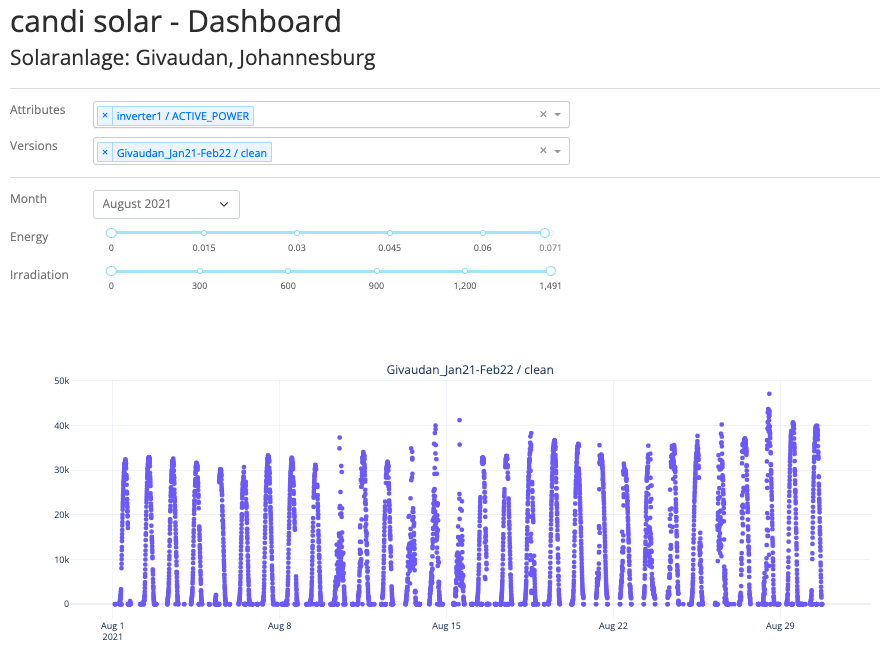
\includegraphics[width=0.2\textwidth]{./dashboard.png}
    \caption{Initial view of dashboard.}
    \label{dashboard}
\end{wrapfigure}

\subsection{Dashboard Example}

To demonstrate these principles, the dashboard with the solar power plant data is used (see Figure \ref{dashboard}). The goal of it is to allow the viewer inspecting the variables that are of interest for them. Therefore, they must first select them from the dropdown at the top of the dashboard. Afterwards, the dashboard shows the values over time in a line chart with a line for each selected variable. There, the user can get an overview of the data for the current month.

\begin{wrapfigure}{R}{0.2\textwidth}
    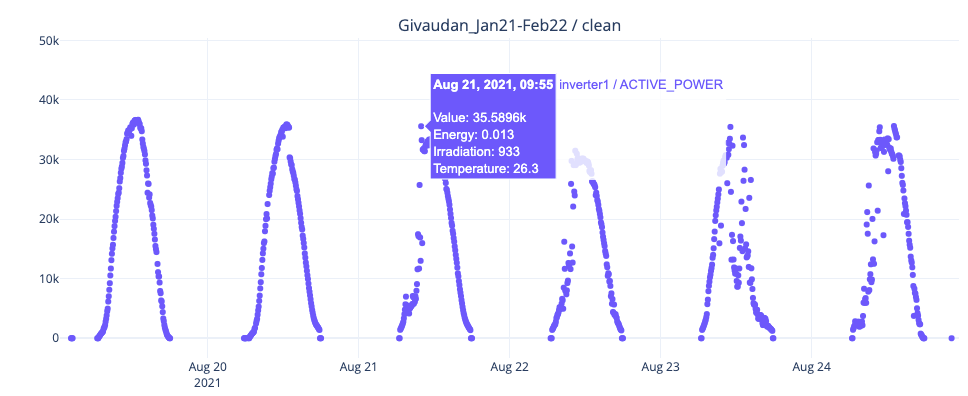
\includegraphics[width=0.2\textwidth]{./dashboard-details.png}
    \caption{Dashboard showing details-on-demand.}
    \label{dashboard-details}
\end{wrapfigure}

Zooming is possible by selecting the desired area by pressing and moving the cursor directly in the plot. The visualisation can be reset to the complete data by double-clicking on it. Lines can be temporarily hidden from the dashboard by clicking on the corresponding attribute name on the right-hand side, or only a specific attribute can be displayed by double-clicking on its name. The data can also be filtered by variables not shown in the plot. Sliders can be used to narrow the range of desired values for energy and irradiation.

\begin{wrapfigure}{R}{0.2\textwidth}
    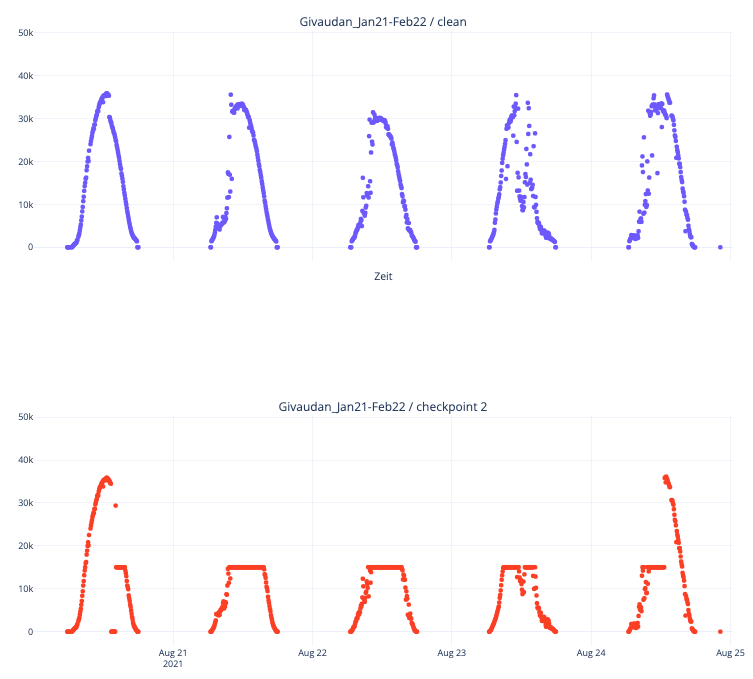
\includegraphics[width=0.2\textwidth]{./dashboard-brushing.png}
    \caption{Dashboard applying principle of brushing.}
    \label{dashboard-brushing}
\end{wrapfigure}

The details of a particular data point can be obtained by pointing the cursor over it. A box will be rendered with the timestamp and the exact values of it. Additional attributes such as energy, irradiation and temperature are also displayed in this tooltip. An example is shown in Figure \ref{dashboard-details}.

This dashboard also supports the comparison of the data after the various cleansing steps to validate the changes. The user can choose the versions of the data they want to compare and a new plot is created for each selected version. As the data come from the same source, they are connected and brushing is applied to the plots. The automatically aligned axes after zooming into the data can be seen in Figure \ref{dashboard-brushing}. Filters and zoom level is propagated to all of them. However, an improvement for the dashboard would be to visually link the data points.

This dashboard is used by data scientists to familiarise themselves with the data they have received. Once the domain knowlegde and data understanding has been acquired, the dashboard might lose its relevance. Nevertheless, it is reasonable to apply these principles to a temporary dashboard as well.

\pagebreak
\section{Human Computer Interaction Basics}

When creating an interactive visualisation, whether it is part of a dashboard or not, the guidelines for static charts should be followed as described by \textcite{weibel_fundamentals_2021}. In addition, there are specific principles for human interactions with computers, and since an interactive visualisation falls into this category, these should also be followed. They ensure that the chart works as the user intends. \textcite{dimara_what_2020} define what an interaction is in data visualisation:

\begin{quote}
    Interaction for visualization is the interplay between a person and a data interface involving a data-related intent, at least one action from the person and an interface reaction that is perceived as such ~\parencite{dimara_what_2020}.
\end{quote}

\subsection{Interaction Laws}

Most of these guidelines originate from psychologisists who have studied interaction behaviour and have been able to summarise it into general laws. These laws are not only applied to data visualisation, but more generally to the design of user interfaces.

\textbf{Miller's Law} states that a human can retain up to seven items (±2) in working memory \parencite{miller_magical_1956}. Contrary to the opinion of many designers, he never concluded that the number of items must be limited to about seven. Instead, he proposed a technique called chunking \parencite{yablonski_millers_2020}. Since the size of an item has no effect on memorability, a large number of items can be divided into meaningful groups to make it easier for the brain to memorise. For example, a phone number or a credit card number can be split up according to a common chunk pattern.

\begin{multicols}{2}
    \noindent
    $$0112345813 \rightarrow 011\;234\;58\;13$$
    $$2222410740360010 \rightarrow 2222\;4107\;4036\;0010$$
\end{multicols}

\begin{wrapfigure}{R}{0.15\textwidth}
    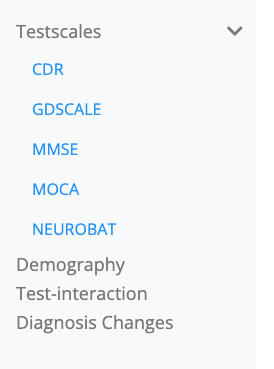
\includegraphics[width=0.15\textwidth]{./menu-collapsible.png}
    \caption{The dashboard's navigation items are structured hierarchically.}
    \label{menu-collapsible}
\end{wrapfigure}

A similar problem is addressed by \textbf{Hick's Law}. According to that, the time it takes humans to make a decision depends on the number of options they have to choose from. The fewer options, the faster the decision is made \parencite{soegaard_hicks_2020}. Reducing the number of options is one possible solution. However, in certain situations it makes more sense to group them in a hierarchical structure to make it easier for the user to find the option they are looking for. In some cases, a user interface may contain features that are only interesting for expierienced users or those with strong knowledge about the data and the tool. To keep the interface simple for normal users, these functions can be hidden by default, and instructed users can show them via a special view or by pressing a special button.

The number of navigation items in the dashboard for the ADNI data grew steadily during the development phase. To counteract the increasing complexity described by Miller and Hick, the navigation items were restructured into a hierarchy, with items from the second level onwards initially hidden. The first level and each sub-level contains no more than seven options and the user is guided to their choice (see Figure \ref{menu-collapsible}).

\textbf{Fitts' Law} describes the relationship between the time it takes to move a pointer to a given target, with two findings interesting for HCI. It states that the greater the distance between the initial position of the pointer to the position of the target, the longer the pointer takes. The size of the target has also an impact on time. The smaller it is, the longer it takes the user to reach the area, because the smaller it is, the more the movement speed has to be reduced in order not to overshoot the target \parencite{budiu_fittss_2022}. A pointer can be a mouse cursor or a finger for touch input. It could be that with a cursor the target's size has a greater influence than with a finger, as it more difficult to control a mouse than your own hand.

Optimal user interfaces and thus interactive visualisations ensure that related components are close together and that all clickable areas are large enough to be clicked without having to reduce the pointer's speed too much. For touch input, it is advisable to add extra padding to clickable areas to increase error tolerance, as human fingers might miss the area slightly \parencite{hoober_fitts_2022}.

\begin{wrapfigure}{R}{0.15\textwidth}
    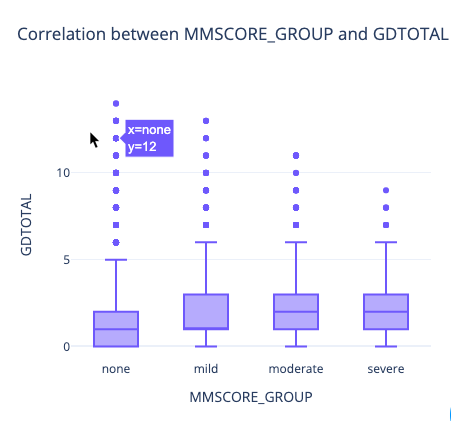
\includegraphics[width=0.15\textwidth]{./fitts-cursor.png}
    \caption{Popover is shown for the marker closest to the cursor.}
    \label{fitts-cursor}
\end{wrapfigure}

Common charts such as scatter plots, line charts and box plots display the data or parts of it as small markers. Interactive variants of these usually show exact values and additional information when these markers are hovered over, which is not optimal as they are very difficult to reach. A solution to this problem could be to add extra padding around each marker. This can either be a fixed amount, or the free space is distributed evenly among the markers in the area \parencite{mccrocklin_interaction_2015}. However, the first approach is easier to implement but raises a problem with overlapping padding areas. Anyway, the extra padding allows the user to point only near the marker and they do not really need to slow down. In both dashboards, the latter approach was implemented, as shown in a box plot in Figure \ref{fitts-cursor}.

\subsection{Transitions}

But not only the human's action should be optimised. They should also receive an appropriate reaction from the user interface that their action has been received and the action is being processed. This is especially crucical if the result of user's triggered action does not become immediately visible. At least a spinner animation should be shown in such cases (see chapter on performance). The user needs to know if they really triggered the action or if they have to try again.

In many cases, the user interface changes after an interaction. To help the user understand what is happening and to check that the interface is behaving as intended, animated transitions between the states of the views can be useful. It is important that the animation reflects the transition and that the animation feels natural. If the user has selected an area to zoom in on, the transition to the zoomed area can be made by steadily increasing the size of the selected area until it reaches the size of the chart. In this way, the human can understand that the chart now shows exactly the selected area.

\subsection{Accessibility}

In Switzerland, every fifth inhabitant is impaired by a disability \parencite{federal_statistical_office_persons_2019}. It is therefore very likely that an interactive visualisation will be used by someone who has problems with it unless special optimisations are made. Colour blindness needs to be taken into account when choosing colours and the visualisation needs to be optimised for screenreaders. This by telling them the function of each interactive component. In web-based implementations, this can be achieved by using the WAI-ARIA framework \parencite{nurthen_wai-aria_2022}.

\subsection{Advanced Interaction Techniques}

For many years now, the computer mouse and touch gestures were the main interaction techniques. However, new and more advanced techniques such as voice input and hand gestures are becoming more popular and might also be used to interact with visualisations. These offer simplicity to users but might lead to new challenges for data scientists and developers. Virtual reality allows data to be expierienced in 3D, and users can walk through the data. And hand gestures will allow them to select specific data points more precisely. Voice control will amke filtering and zooming easier, but selecting individual data points will be more difficult if they can not be addressed with an identifier.

\pagebreak
\section{Evaluation}

\begin{wrapfigure}{R}{0.3\textwidth}
    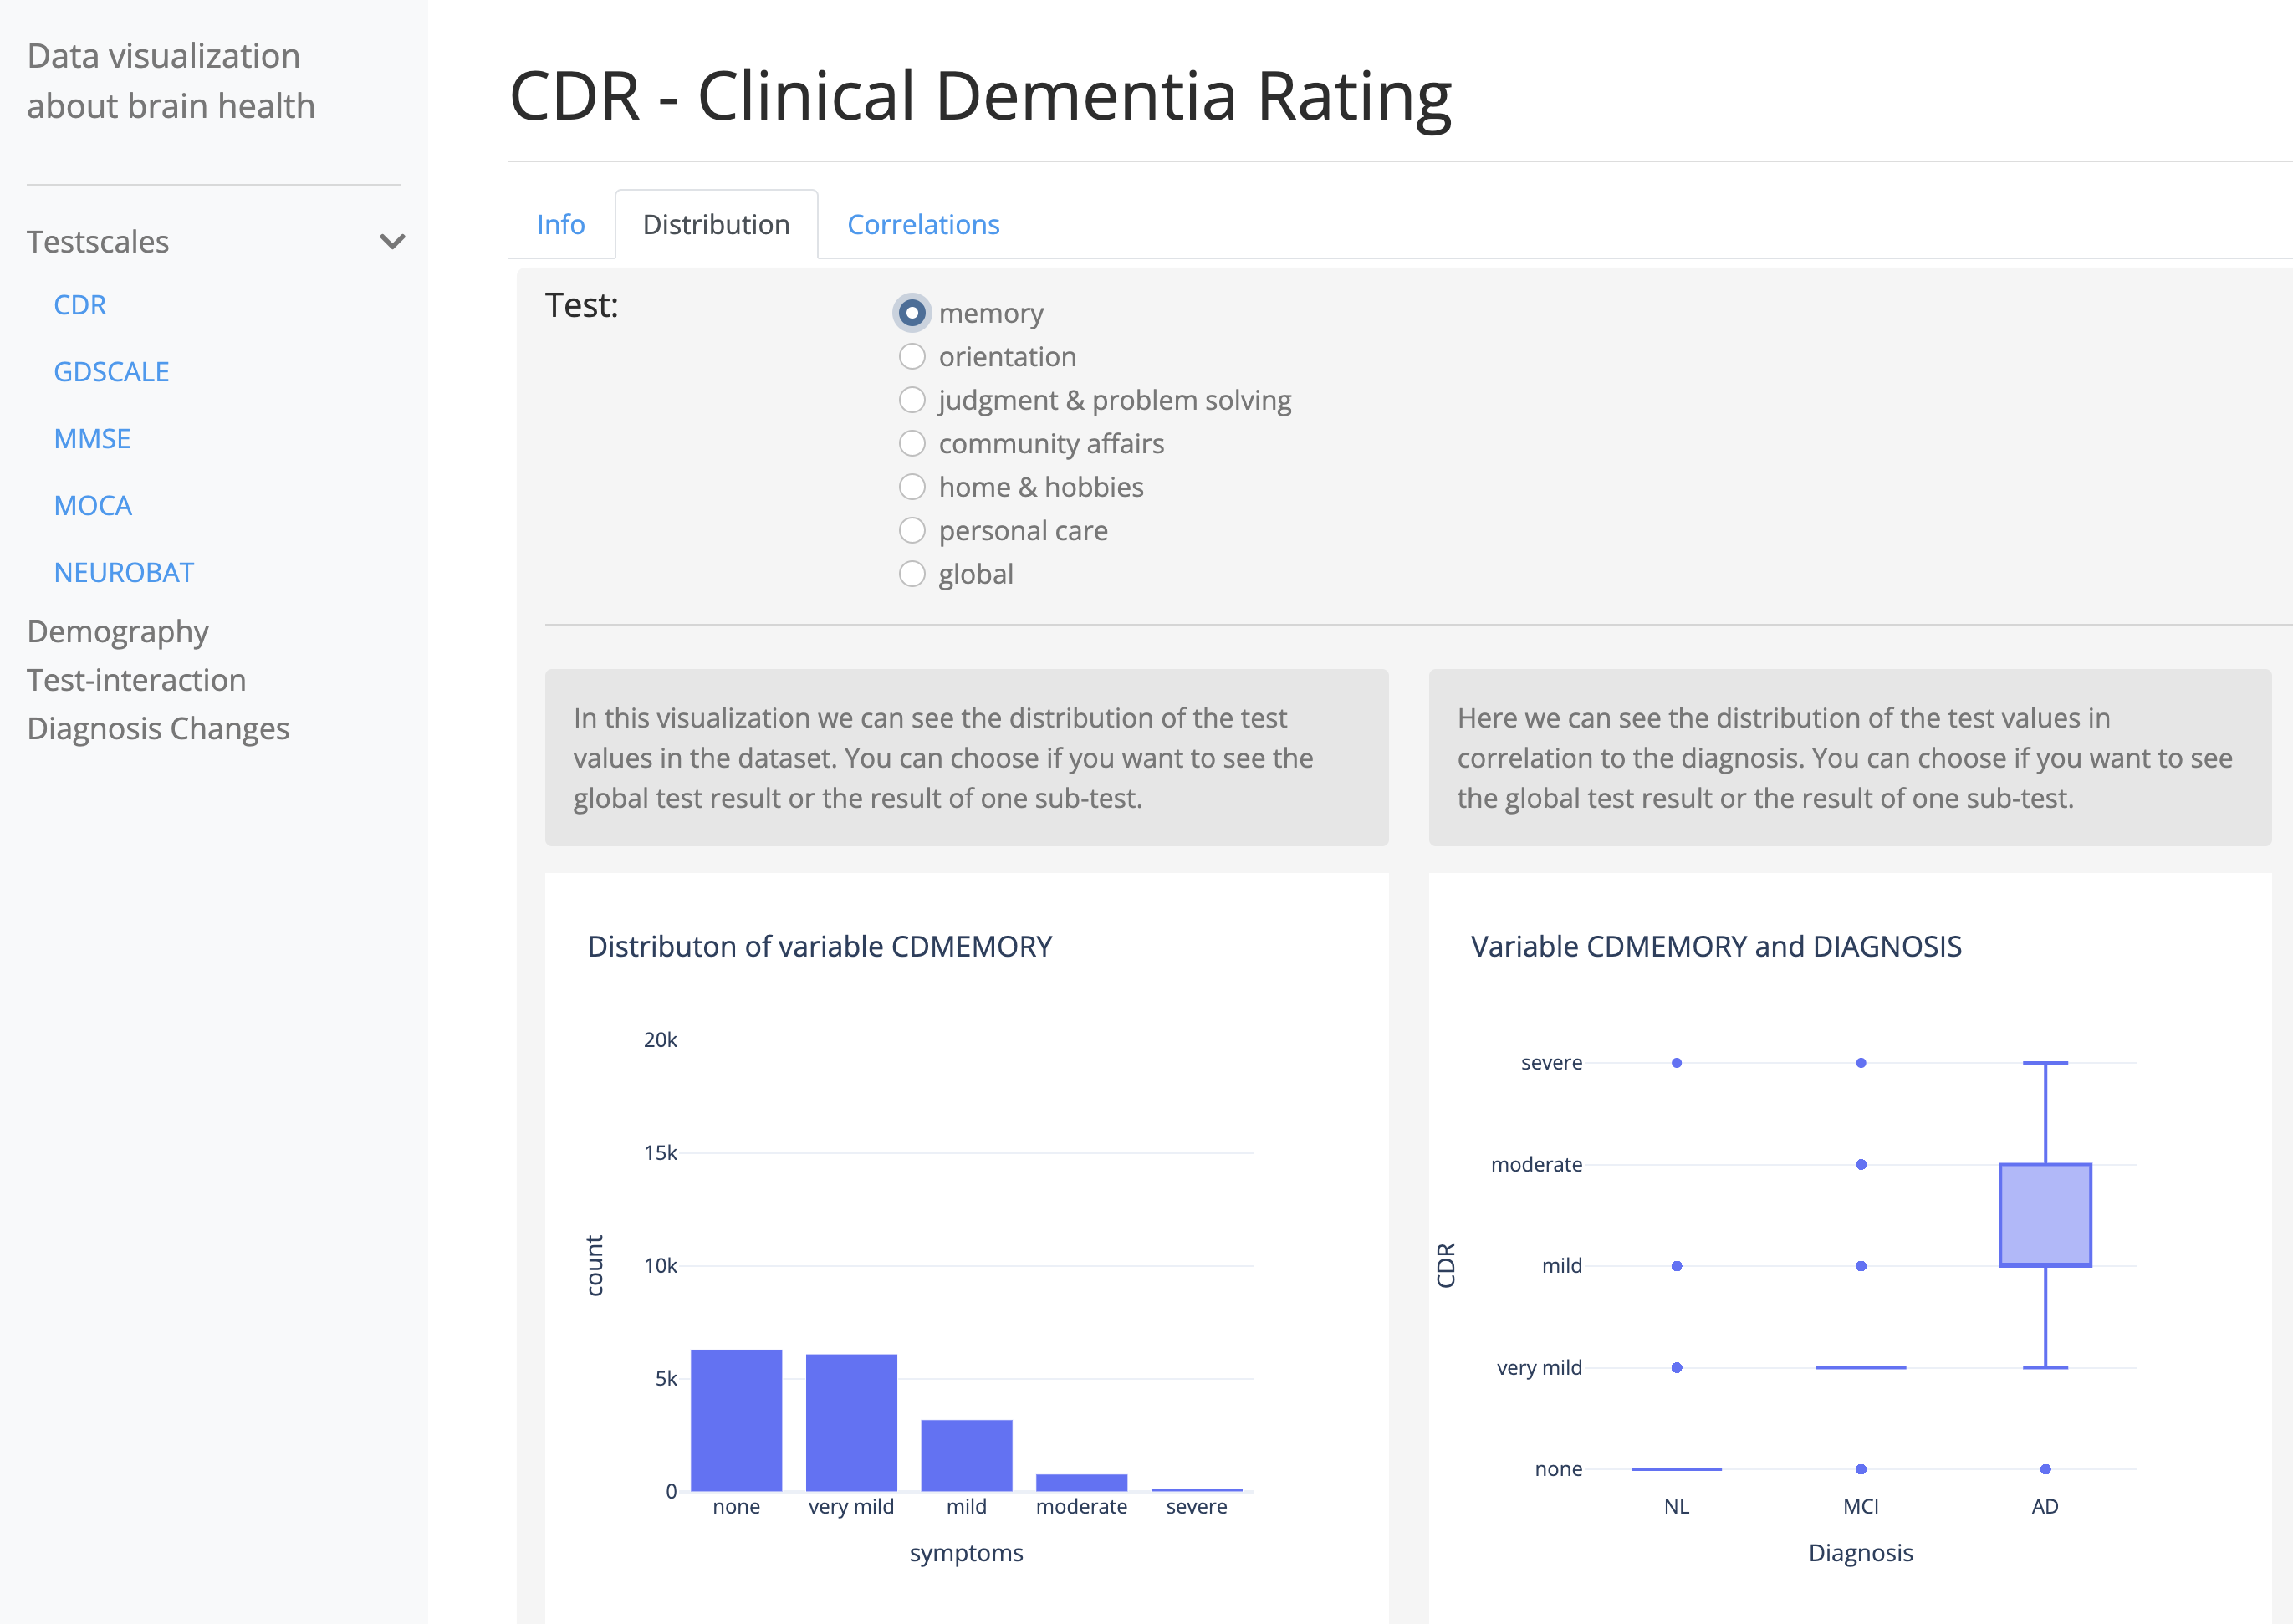
\includegraphics[width=0.3\textwidth]{./adni-cdr.png}
    \caption{View in the ADNI dashboard showing distributions of the CDR testscale.}
    \label{adni-cdr}
\end{wrapfigure}

Like static data visualisations, interactive ones should be evaluated to verify that they serve the intended purpose in a user-friendly manner. Evaluations can basically be performed in the same way as for static plots and are outlined by \textcite{weibel_fundamentals_2021}. However, they tend to be more extensive because interactivity allows more actions that can be reviewed.

Since an interactive visualisation is not just an image but a software product, the same testing routines apply here as well. All functionality should be tested either manually or using test automation software. In the case of a web application, the visualisation should be tested in all browsers used by the viewers.

\subsection{Conducting an Evaluation}

An evaluation was conducted for the ADNI data dashboard to determine if it is serving its purpose. To do this, evaluation participants were asked to answer five questions for which the dashboard was developed. As they searched for the solutions, their behaviour was observed to identify potential hurdles and problems.

\begin{itemize}
    \item How many subjects participated in the ADNI study and what are their diagnosises?
    \item Which CDR subscale correlates most strongly with the diagnosis?
    \item What is the median value of RAVLT immediate for subjects with CDGLOBAL none?
    \item What is the correlation between MOCA and GDTOTAL?
    \item How many subjects transitioned from AD to MCI and from MCI to AD during the study?
\end{itemize}

\begin{wrapfigure}{R}{0.3\textwidth}
    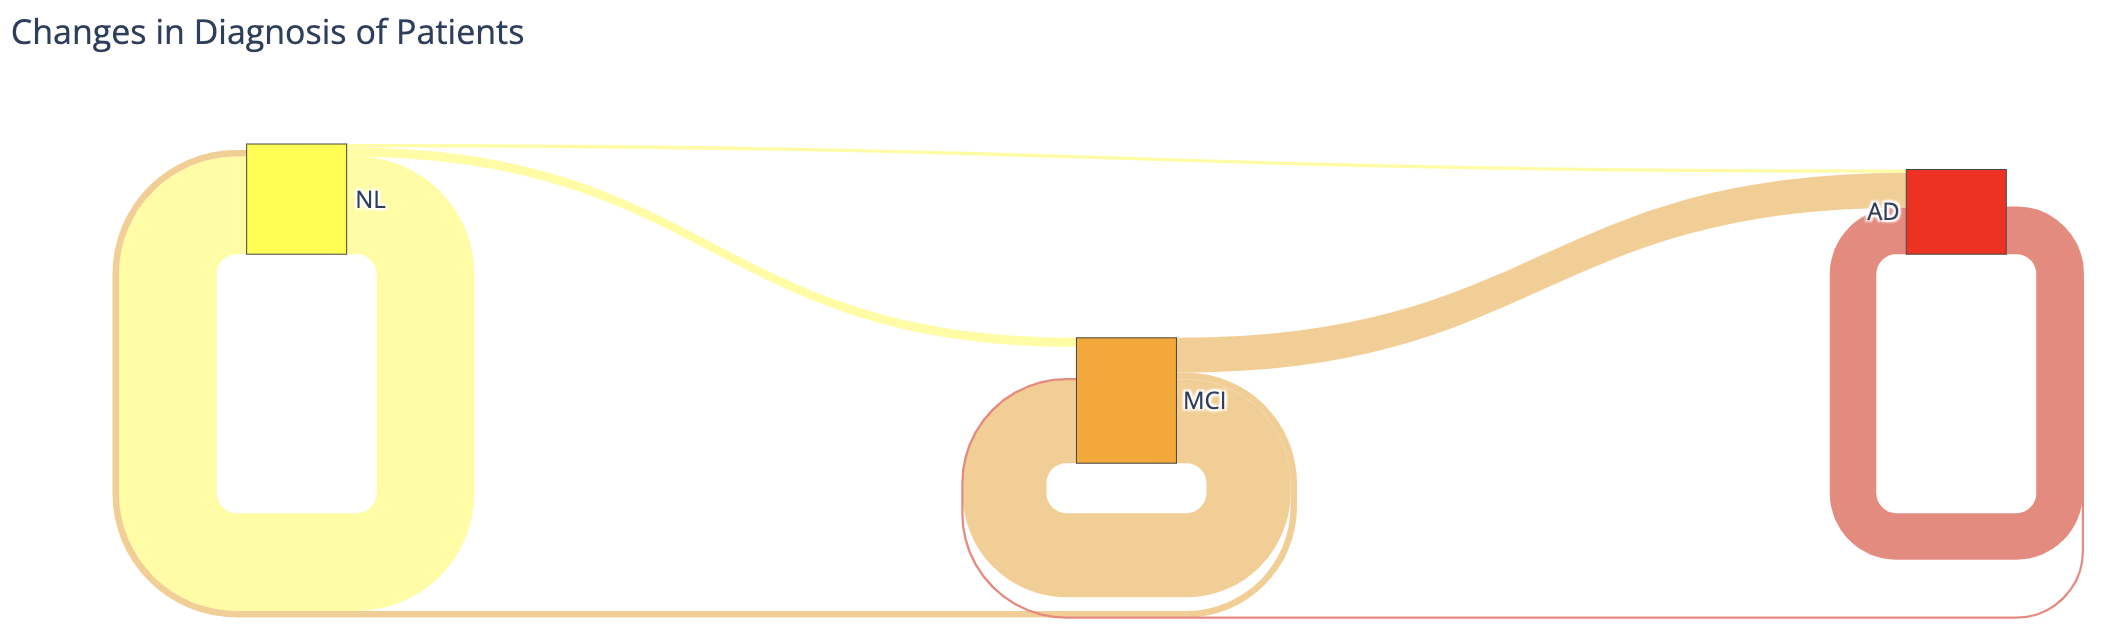
\includegraphics[width=0.3\textwidth]{./sankey.png}
    \caption{Sankey plot showing changes in subject's diagnois during ADNI study.}
    \label{sankey}
\end{wrapfigure}

These five tasks cover most parts of the dashboard and involve finding values in different kinds of visualisations. Some of the answers are part of interactive plots, where the searched value will appear only when the mouse is hovered over a specific area. Other results are part of short texts that can be found on the right page and tab. For some questions the answer can be found in several places. For example, the numbers for the last question are listed in a table and also visualised in an interactive Sankey plot (see Figure \ref{sankey}).

Since the target audience for this dashboard consists of data scientists, all participants have knowledge in this area and are familiar with the concepts of distributions and correlations. However, all participants will be introduced into the ADNI data and given necessary domain knowledge as this is required to understand the information on the dashboard.

The evaluation was conducted one at a time with three data scientist students who had never seen the dashboard before. After the introduction, they were given one task at a time. Interestingly, all of them had very different strategies for answering the five questions. One person tried to get an overview of the dashboard first and did not seem to hurry. The others tried to find the answers as quickly as possible. One of them clicked through all navigation items with no apparent strategy. The last person tried to figure out under which navigation item the answer might be located. Depending on their strategy, they took different amounts of information from the dashboard. Nevertheless, all of them were able to answer the questions correctly in adequate time. It took them between 7 and 15 minutes, depending on how they proceeded.

\subsection{Improvements}

By observing the participants as they tried to find the answers, some problems were discovered in the dashboard. Also, interviewing the participants after the evaluation confirmed and revealed further issues they faced during their tasks. Aside from the fact that all of them were able to complete the tasks, these inputs are the most important information provided by such an evaluation.

The navigation items were not understandable enough for all participants. One person had not realised that there were subordinate navigation items which were only shown when clicked on the parent item. There was a small arrow next to it indicating this behaviour. However, this did not seem to be sufficient. The navigation item with the name "Diagnosis Changes" was misleading to everyone, as they assumed it to be the progression of the participants' diagnosis. However, under this item, the impact of each testscale variable on diagnosis change was examined. The actual number of changes was visualised on another page. Adding a link to this page to the expected one or renaming the navigation could solve that issue.

\begin{wrapfigure}{R}{0.2\textwidth}
    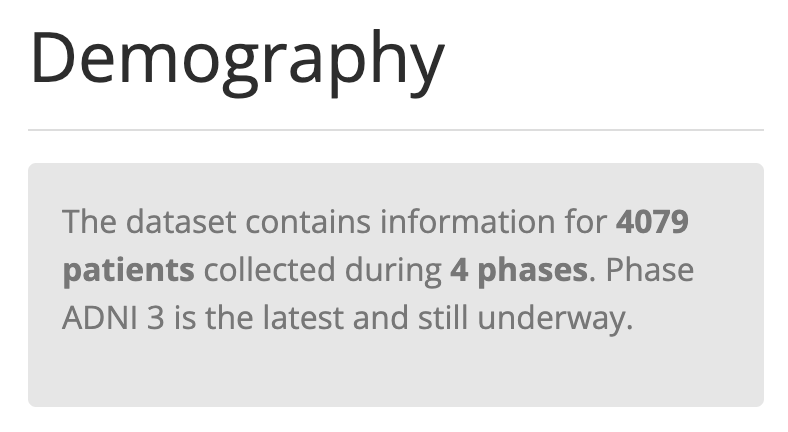
\includegraphics[width=0.2\textwidth]{./info-in-text.png}
    \caption{Highlighted data in text.}
    \label{info-in-text}
\end{wrapfigure}

The evaulation also showed that extracting information from continuous text is not as easy as extracting it from table and visualisations. It might be beneficial to convert the texts in the dashboard into tables listing the data, or at least to highlight the numbers in them by marking them bold, for example (see Figure \ref{info-in-text}). In addition, different visualisations were actaully used to answer the questions. Some also generally preferred tables to charts.

The Sankey plot indicating diagnosis changes was met with controversy. None of the participants needed an introduction to this unconventional plot, but some stated at the end of the evaluation that they would have preferred a simpler visualisation. This shows that even some data scientists prefer the classic visualisation to a specialised one. Finally, the subject of the dashboard prooved difficult to understand. What was desired was a written introduction and an overview for the different test scales. According to one participant, this would have made it easier to get started with the dashboard.

\section{Conclusion}

Knowing about the basic design principles and psychological laws is useful to understand how visualisations are perceived by humans. However, once there is an idea how an interactive visualisation should be created, it is often very helpful to create a prototype of the theoretical concept. With such a prototype, it quickly becomes clear whether the idea really works. Then it is also possible to conduct an evaluation with the users of the target audience to verify whether they understand and are able to use the visualisation. The longer one waits with such an evaluation, the more time is wasted in case there are fundamental problems with the visualisation design. Several short iterations of design, implementation and evaluation will ensure a product that end users will love.

Interactive visualisations are a powerful tool to bring complex data understandable for people. But creating them is also complex and many concepts need to be considered when designing such a visualisation. Fortunately, there are several libraries that already apply many of these concepts. Repetitive implementation tasks such as zooming and filtering can be delegated to the libraries. This allows data scientists to focus on the exciting parts of their job and mostly domain-specific questions, such as finding the right chart type for the data.

\pagebreak
\section{Appendix}
Lorem Ipsum

\pagebreak
\printbibliography


\end{document}
